%% LyX 2.0.0 created this file.  For more info, see http://www.lyx.org/.
%% Do not edit unless you really know what you are doing.
\documentclass[french,english]{article}
\usepackage[T1]{fontenc}
\usepackage[latin9]{inputenc}
\usepackage{array}
\usepackage{multirow}
\usepackage{amsmath}
\usepackage{amssymb}
\usepackage{graphicx}

\makeatletter

%%%%%%%%%%%%%%%%%%%%%%%%%%%%%% LyX specific LaTeX commands.
%% Because html converters don't know tabularnewline
\providecommand{\tabularnewline}{\\}

%%%%%%%%%%%%%%%%%%%%%%%%%%%%%% User specified LaTeX commands.
% Template for ICIP-2012 paper; to be used with:
%          spconf.sty  - ICASSP/ICIP LaTeX style file, and
%          IEEEbib.bst - IEEE bibliography style file.
% --------------------------------------------------------------------------

\usepackage{spconf}

% Example definitions.
% --------------------
\def\x{{\mathbf x}}
\def\L{{\cal L}}

\usepackage{babel}\addto\extrasfrench{%
   \providecommand{\og}{\leavevmode\flqq~}
   \providecommand{\fg}{\ifdim\lastskip>\z@\unskip\fi~\frqq}
}



\usepackage{babel}\addto\extrasfrench{%
   \providecommand{\og}{\leavevmode\flqq~}
   \providecommand{\fg}{\ifdim\lastskip>\z@\unskip\fi~\frqq}
}


\name{Luiza Orosanu, Denis Jouvet, Dominique Fohr, Irina Illina, Anne Bonneau\thanks{The work presented in this article is part of the ALLEGRO project, funded by the European program INTERREG IV.}}
\address{Speech Group, LORIA\\
Inria, Villers-les-Nancy, F-54600, France\\
CNRS, LORIA, UMR 7503, Villers-les-Nancy, F-54600, France\\
Universite de Lorraine, LORIA, UMR 7503, Villers-les-Nancy, F-54600, France\\
{\small \tt \{luiza.orosanu, denis.jouvet, dominique.fohr, irina.illina, anne.bonneau\}@loria.fr }}

\makeatother

\usepackage{babel}
\addto\extrasfrench{%
   \providecommand{\og}{\leavevmode\flqq~}
   \providecommand{\fg}{\ifdim\lastskip>\z@\unskip\fi~\frqq}
}

\begin{document}

\title{Combining criteria for the detection of incorrect entries of non-native
speech in the context of foreign language learning}
\maketitle
\begin{abstract}
This article analyzes the detection of incorrect entries of non-native
speech in the context of foreign language learning. The purpose is
to detect and reject incorrect entries (i.e. those for which the speech
signal does not correspond at all to the associated text) while being
tolerant to the mispronunciations of non-native speech. The proposed
approach exploits the comparison between two text-to-speech alignments:
one constrained by the text which is being checked, with another one
unconstrained, corresponding to a phonetic decoding. Several comparison
criteria are described and combined via a logistic regression function.
The article analyzes the influence of different settings, such as
the impact of non-native pronunciation variants, the impact of learning
the decision functions on native or on non-native speech, as well
as the impact of combining various comparison criteria. The performance
evaluations are conducted both on native and on non-native speech. 
\end{abstract}
\begin{keywords} Foreign language learning, incorrect entries, non-native
speech, constrained and unconstrained alignments \end{keywords}


\section{Introduction}

\label{sec:intro}

Support for foreign language learning is an application area of automatic
speech recognition technologies. Their objective is to detect and
to provide feedback on pronunciation errors, in order to help correcting
them and slowly improve the foreign language proficiency. One of the
main difficulties for such a system is to automatically detect and
locate pronunciation errors \cite{Herron99automaticlocalization},
while remaining robust to non-native speech. Several methods have
been proposed to determine a score for the pronunciation quality \cite{Witt200095},
by exploring likelihood ratios. Such systems benefit from the introduction
of acoustic models of native phonemes (in addition to those belonging
to the target language), along with the a priori knowledge of possible
non-native mispronunciations.

The prosody is an other important element of foreign language learning.
Some projects have addressed the feedback on duration errors \cite{Eskenazi00thefluency}.
An original method was proposed in \cite{foreignLanguage}, which
aims to improve both production and perception, by combining an accurate
and detailed prosodic feedback with an audio feedback based on a modification
of the learner's pronunciation. This approach requires a phonetic
segmentation of the learner's utterance; a study of the relevance
of the phonetic segmentation has been undertaken in \cite{MESBAHI_Reliability}.
These automatic methods for pronunciations diagnosis are based on
a phonetic segmentation of the speech signal, which is obtained via
a forced alignment with the models corresponding to the pronounced
sentence. The inclusion of non-native pronunciation variants improves
the quality of alignments \cite{nonNative}.

However, the learner does not always pronounce (entirely or at all)
the sentence requested by the learning exercise (error of pronunciation,
speech interference, sound capture issue, ...). Hence, before analyzing
the quality of the learner's pronunciation or even working on obtaining
a relevant prosodic feedback, the system must be able to determine
if the audio signal actually corresponds to the expected sentence.
So, the objective of this study is to detect and to reject incorrect
entries. With this kind of filtering, we can be sure that the data
on which we will be working on is acceptable (or maybe even 100\%
correct), and thus further detailed processing and analysis will be
relevant.

In speech recognition, such a decision typically corresponds to the
detection of out-of-vocabulary words or of sentences that do not contain
any key words \cite{outOfVocabulary,boite2000traitement}. Unlike
these approaches, which mainly aim the native speech, here we want
to offer support for foreign language learning, and thus we need to
detect obvious inconsistencies (i.e. an audio signal that does not
correspond to the expected sentence), but at the same time tolerate
non-native mispronunciations.

Thus, this article performs a detailed study on the rejection of incorrect
entries in the context of foreign language learning. The paper analyzes
the impact of various comparison criteria, both on native and on non-native
speech. The first section provides a description of our methodology,
in particular the criteria used to distinguish correct entries from
incorrect ones, along with the chosen classifier. The second part
of the paper is devoted to the description of experiments and the
discussion of results.


\section{Methodology}

\label{sec:Methodology}

In order to reject incorrect entries, while accepting those that are
correct, we must determine whether or not the audio signal corresponds
to the expected sentence. For that, a decision was taken: to decode
the audio signals in three different ways (one constrained alignment,
and two unconstrained decodings) and to compare the resulting phonetic
segmentations.


\subsection{Phonetic segmentations}
\begin{enumerate}
\item Constrained decoding (forced alignment)\textit{:} the system is forced
to follow the sequence of words within the expected text. 
\item Phonetic decoding based on phoneme loop: the system is free to choose
any phoneme in any position in the sentence. 
\item Phonetic decoding based on word loop: the system is free to choose
any word (limited to the \textasciitilde{}200 words of the learning
application) in any position in the sentence. 
\end{enumerate}
For the segmentations (1) and (3), the words may have several pronunciation
variants, native and/or non-native, according to the associated lexicon.


\subsection{Comparison criteria\label{sub:Decision-criteria}}

The comparison criteria serve to distinguish correct entries from
incorrect ones. They are based on information extracted from the constrained
and unconstrained segmentations. Two comparisons are made: first one
between the segmentations (1) and (2) ({}``phoneme loop comparison''),
and the second one between the segmentations (1) and (3) ({}``word
loop comparison''). The comparison takes into account the phonemes,
the frames, the non-speech segments, the likelihood ratios or the
phoneme durations. 
\begin{enumerate}
\item Criterion associated to the phonemes\label{enu:Criterion1}: percentage
of phonetic segments that have the same label in both segmentations
and where starting or ending temporal boundaries are within a 20ms
interval. The non-speech segments are ignored. This criterion is generally
greater for correct entries than for incorrect ones. 
\item Criterion associated to the frames\label{enu:Criterion2}: percentage
of frames whose labels belong to the same phonetic class in both segmentations.
A phonetic class is represented by sounds which share at least one
phonetic feature, and especially the \textquotedbl{}manner of articulation\textquotedbl{}
(e.g stop class, fricative class, ...). Even if the phonetic decoding
does not always find the correct phoneme, it is likely to replace
it with another one belonging to the same class. This criterion is
generally greater for correct entries than for incorrect ones. 
\item Criterion associated to the non-speech segments\label{enu:Criterion3}:
duration difference of non-speech segments between the two segmentations
(as a percentage of the total duration of the utterance). When the
system is forced to align an audio signal on a non-matching text (the
case of an incorrect entry), it is likely to add several non-speech
segments between words and / or increase or decrease the duration
of those that actually exist. This criterion is generally smaller
for correct entries than for incorrect ones. 
\item Criterion associated to the \textit{log} likelihood ratio\label{enu:Criterion4}:
difference between the logarithmic likelihoods of both segmentations.
A value close to {}``0'' indicates that both segmentations lead
to the same logarithmic likelihood, which means that they correspond
to the same sequence of phonemes (a correct entry). The log likelihood
ratio gets smaller (negative value) for incorrect entries. 
\item Criterion associated to the phoneme durations\label{enu:Criterion5}:
difference between the number of short phonemes (having the minimal
duration of exactly 3 frames which corresponds to the 3 emitting states
of the HMM, Hidden Markov Model) within both segmentations (as a percentage
of the total number of phonemes within the forced alignment). A significant
quantity of phonemes with minimal durations could indicate abnormalities
within the alignment. This criterion is generally smaller for correct
entries than for incorrect ones. 
\end{enumerate}
\begin{figure*}[t]
\centering{}\includegraphics[scale=0.43]{Image/courbeDET_EnglishTest_lex_training}\hspace{0.5cm}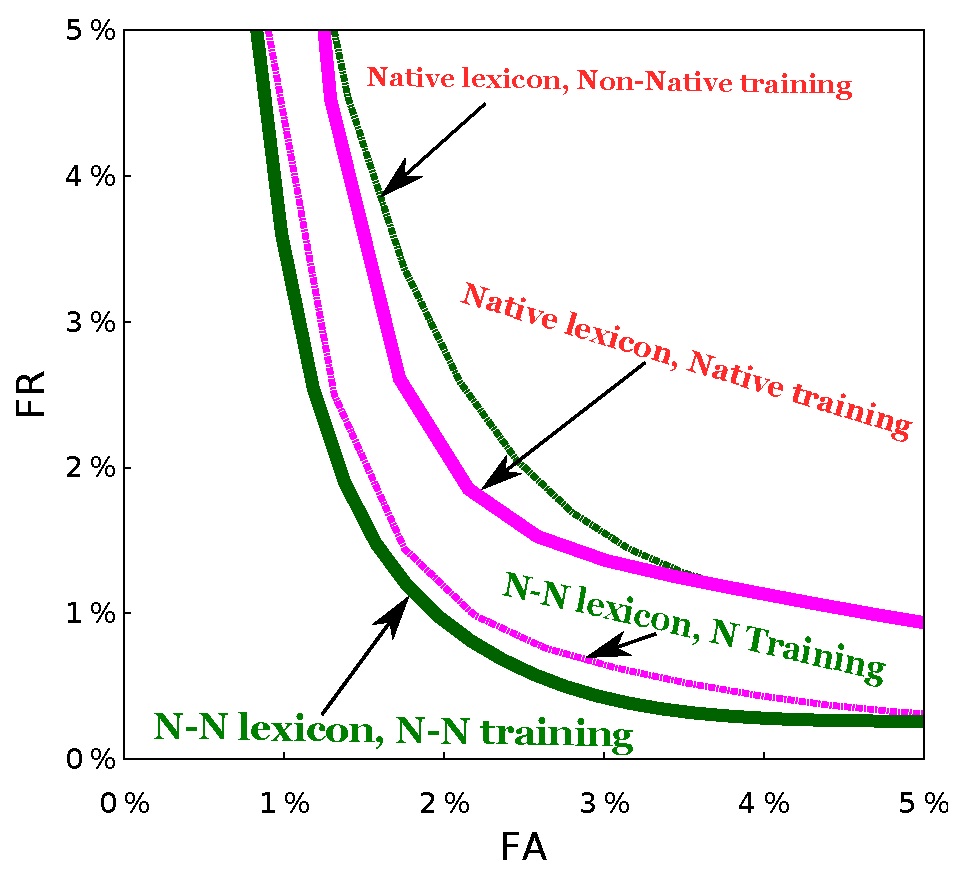
\includegraphics[scale=0.43]{Image/courbeDET_MAC_lex_training}\caption{Impact of lexicon and training data on DET curves for native data
(a) and for non-native data (b), when incorrect entries are represented
by entirely modified transcriptions and when using 10 comparison criteria}
\label{Figure1}
\end{figure*}



\subsection{Data classification}

Given the comparison criteria (section \ref{sub:Decision-criteria})
and the classification task limited to two classes (correct or incorrect),
the predictive model of the logistic regression \cite{Dreiseitl2002352}
was chosen as binary classifier. The logistic regression is used here
to compute an entry's probability of being correct:

\selectlanguage{french}%
\textbf{
\begin{equation}
f(\overline{X})=\frac{1}{1+exp(-(\alpha_{0}+\alpha_{1}x_{1}+\ldots+\alpha_{10}x_{10}))}
\end{equation}
}

\selectlanguage{english}%
The first step of the approach is to train the parameters of the classifier
on the training data. The training data is represented by the data
set \foreignlanguage{french}{ 
\[
D=\left\{ \overline{X_{i}},\: y_{i}\right\} ,\: i=1,...,N
\]
} where: 
\selectlanguage{french}%
\begin{itemize}
\item $\overline{X}=<x_{1},x_{2},\ldots,x_{10}>$\foreignlanguage{english}{is
the vector containing the entry's informations, in other words the
comparison criteria (10 in total)}
\selectlanguage{english}%
\item $y$ indicates the membership in the correct class ($y=1$) or in
the incorrect one ($y=0$) 
\item $N$ is the number of entries within the training data set. 
\end{itemize}
\selectlanguage{english}%
We train the unknown $\alpha=(\alpha_{0},\alpha_{1},\ldots,\alpha_{10})$
parameters by minimizing the error function $E$. The error function
indicates the mismatch between the class membership (which is either
0 or 1) and the $f(\overline{X})$ value of the logistic function
which varies between 0 and 1.



\selectlanguage{french}%
\begin{center}
\textbf{
\begin{equation}
E=-\overset{N}{\underset{i=1}{\sum}}\left(y_{i}\cdot ln\left(f(\overline{X_{i}})\right)+\left(1-y_{i}\right)\cdot ln\left(1-f(\overline{X_{i}})\right)\right)
\end{equation}
}
\par\end{center}

\selectlanguage{english}%
The minimization is performed using the gradient descent method. This
numerical algorithm seeks an optimum (possibly local) by successive
improvements. From an $\alpha$ starting point, the parameters are
continuously modified until a stop condition is reached (improvement
smaller than a given threshold).

Then, the DET curves (\textquotedbl{}detection error trade-off\textquotedbl{})
are used to represent the results. A DET curve is an error-rate graphic
for binary classification systems. It is used here to represent the
performance on the task of entries classification, which involves
a compromise between the rates of \textquotedbl{}false acceptance\textquotedbl{}
(\textit{FA}, percentage of incorrect entries classified as correct
by the system) and \textquotedbl{}false rejection\textquotedbl{} (\textit{FR,}
percentage of correct entries classified as incorrect by the system).
An entry is accepted as correct only if the logistic regression's
value $f(\overline{X})$ (for the chosen $\overline{X}$ criteria)
is greater than a threshold $\sigma$. To plot the DET curve, several
values for the threshold $\sigma\epsilon[0,1]$ are considered. The
(FA, FR) error rates for each threshold value are marked on the graphic.
Finally, the best compromise between the error rates (among all the
available points on the DET graphic) is the one that maximizes the
following F-measure:

{\footnotesize 
\begin{equation}
\frac{1}{F}=\frac{1}{2}\cdot\left(\frac{1}{1-FA}+\frac{1}{1-FR}\right)\label{eq:F-measure}
\end{equation}
 }{\footnotesize \par}


\section{Experiments and results}

\label{sec:experiments}


\subsection{Experimental setup}

To evaluate the approaches mentioned in section \ref{sec:Methodology},
two English corpora were used (one native and the other one non-native).
They were both created for the INTONALE project \cite{dargnatMth},
which is devoted to prosodic studies. The native corpora contains
approximately 1500 audio signals, recorded by 22 English speakers
(15 women and 7 men, 66 sentences per speaker). The non-native corpora
contains about 800 audio signals, recorded by 34 French speakers (29
women and 5 men, 23 sentences per speaker). The recordings were made
in a quiet room. The software developed for the recordings displays
a sentence on the screen. The speaker can choose, after each pronunciation
of a sentence, to repeat it (in case of problems) or to move on to
the next.

\begin{figure*}[t]
 

\begin{centering}
\includegraphics[scale=0.43]{Image/courbeDET_EnglishTest_criteria}\hspace{0.5cm}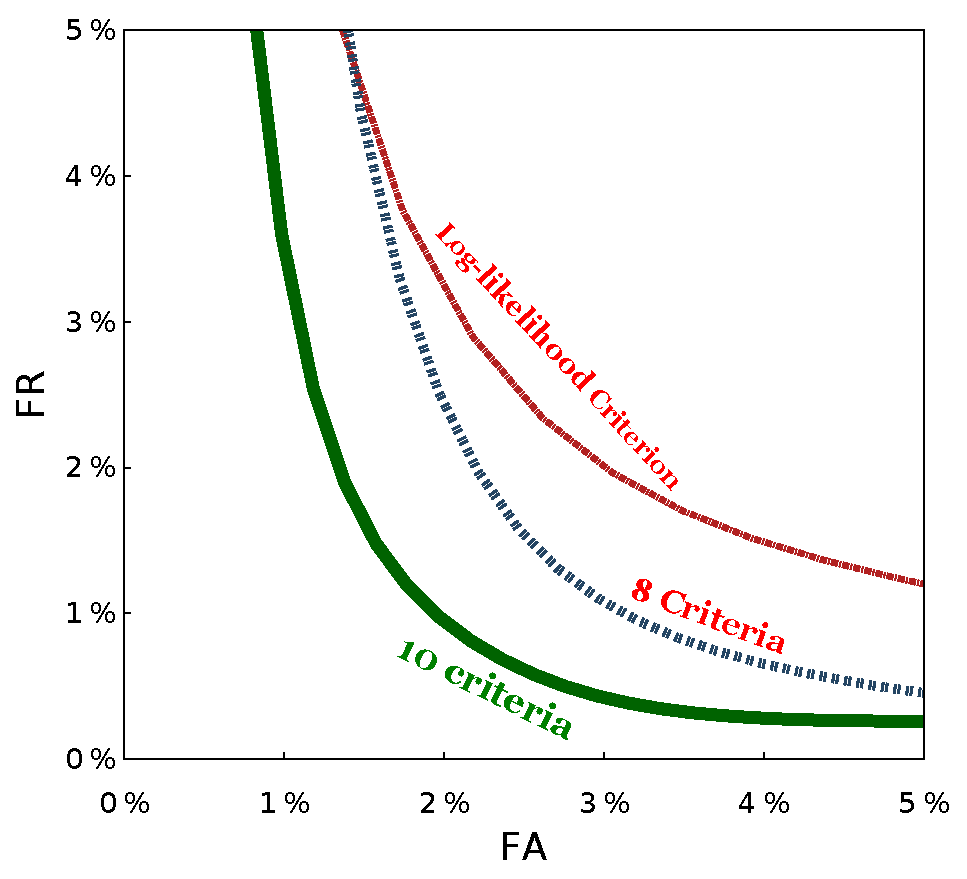
\includegraphics[scale=0.43]{Image/courbeDET_MAC_criteria} 
\par\end{centering}

\caption{Impact of combining various comparison criteria on DET curves for
native data (a) and for non-native data (b), when incorrect entries
are represented by entirely modified transcriptions and when using
native trained parameters and the native lexicon to evaluate native
data and when using non-native trained parameters and the non-native
lexicon to evaluate non-native data}
\label{Figure2}
\end{figure*}


\begin{figure*}[t]
 

\begin{centering}
\includegraphics[scale=0.43]{Image/courbeDET_EnglishTest}\hspace{0.5cm}\includegraphics[scale=0.43]{Image/courbeDET_MAC} 
\par\end{centering}

\caption{Evaluation of DET curves on native data (a) and on non-native data
(b), according to the size of the incorrect part of the entry, when
using 10 comparison criteria and when using native trained parameters
and the native lexicon to evaluate native data and when using non-native
trained parameters and the non-native lexicon to evaluate non-native
data}
\label{Figure3}
\end{figure*}


All used corpora contain only correct entries (even if the non-native
speech is subject to many mispronunciations). To simulate incorrect
entries, we used the same audio signals, but we attached to each of
them a text that does not correspond to it. We modified the transcripts
in two different ways: by replacing a word or a sequence of words
(the sequence of words is extended up to reaching a minimal size of
3 syllables, 4 syllables, 5 syllables, 6 syllables or 7 syllables)
or by replacing the entire sentence. These replacements between words
and between sentences are random. Each corpora, native or non-native,
was divided in two equal parts, one meant to train the parameters,
and the other one to evaluate their performance.

The HTK tools \cite{Young2002} were used to decode the audio signals.
The MFCC (Mel Frequency Cepstral Coefficients) acoustic analysis gives
12 MFCC parameters and a logarithmic energy per frame (window of 32
ms, 10 ms shift). The forced alignment of an entry is done by using
the HMM acoustic models and by taking into account the pronunciation
variants of each word. Each HMM state has been modeled with a 16 Gaussian
mixture. The acoustic models were trained using the TIMIT's English
corpus \cite{timit}. Its audio signals were recorded by 630 U.S.
speakers, with a sampling frequency of 16 kHz. Two lexicons were used:
the first one includes only native variants for each word (native
lexicon: the CMU dictionary \cite{cmu}) and the second one includes
also non-native variants (non-native lexicon). A large number of non-native
pronunciation variants observed in the non-native speech corpora were
included in the pronunciation lexicon (automatic generation of non-native
pronunciation variants gives similar results, but we will not discus
about it in this paper).


\subsection{Evaluation of the lexicon and the training data set}

This section studies the impact of using a native or a non-native
lexicon, along with the impact of using a native or a non-native data
set for training the parameters of the decision function.

Given that it is not possible to know in advance if the pronounced
sentence will be entirely or just partially different from the expected
sentence, we chose to execute a single and global training of the
logistic function, on all our groups of correct \& incorrect data
sets ( {}``3 syllables'' = the group of modified transcripts where
we replaced a word or a group of words having a minimal size of 3
syllables, ..., {}``all syllables'' = the group of modified transcripts
where we replaced the entire sentence). We test it afterwards on each
group separately.

Figure \ref{Figure1} presents the impact of the lexicon and of the
training data set (note that all curves are smoothened and that their
order is indicated in the legend). We report the results obtained
on the {}``all syllables'' data sets, using the combination of all
10 comparison criteria. The curves show that it is important to learn
the decision functions on the same type of data for optimum results.
They also show that the use of non-native pronunciation variants in
the lexicon is necessary for non-native speech. Therefore, the best
results are obtained on native data, with the use of a native lexicon
and training on native data (the \textit{'native training, native
lexicon'} curve in graph (a)), and on non-native data, with the use
of a non-native lexicon and training on non-native data (the \textit{'non-native
training, non-native lexicon'} curve in graph (b)).


\subsection{Evaluation of the comparison criteria}

This section studies the impact of combining various comparison criteria.

Figure \ref{Figure2} presents the impact of different criteria combinations.
The results obtained with a single criterion ( the 'Log-likelihood:
phoneme loop' curve) are improved with the use of the first four criteria
(1, 2, 3 \& 4 in section \ref{sub:Decision-criteria}) computed from
both the phoneme loop and the word loop comparisons (the \textit{'8
Criteria : both loops' }curve). Further improvement is obtained with
the use all 10 criteria (the \textit{'10 Criteria: both loops'} curve).


\subsection{Evaluation of the performance}

This section studies the performance of our classifier.

Figure \ref{Figure3} presents the results obtained on the different
data sets. As expected, the performance increases with the number
of differences between the pronounced sentence and the expected sentence.

\begin{table*}
\begin{centering}
\begin{tabular}{|c|c|r@{\extracolsep{0pt}.}l|r@{\extracolsep{0pt}.}l|r@{\extracolsep{0pt}.}l|c|}
\hline 
\textbf{Data} & \textbf{No. Syll} & \multicolumn{2}{c|}{\textbf{EER}} & \multicolumn{2}{c|}{\textbf{FA}} & \multicolumn{2}{c|}{\textbf{FR}} & \textbf{F-measure}\tabularnewline
\hline 
\hline 
 & 3 & 21&83\% & 20&72\% & 22&51\% & 78.4\%\tabularnewline
\cline{2-9} 
\multirow{4}{*}{\textbf{Native}} & 4 & 15&61\% & 11&46\% & 17&54\% & 85.4\%\tabularnewline
\cline{2-9} 
 & 5 & 14&23\% & 9&39\% & 17&13\% & 86.6\%\tabularnewline
\cline{2-9} 
 & 6 & 11&33\% & 8&56\% & 13&54\% & 88.9\%\tabularnewline
\cline{2-9} 
 & 7 & 9&39\% & 6&08\% & 10&77\% & 91.5\%\tabularnewline
\cline{2-9} 
 & \textbf{all} & \textbf{5}&\textbf{94\%} & \textbf{8}&\textbf{01\%} & \textbf{3}&\textbf{31\%} & \textbf{94.3\%}\tabularnewline
\hline 
\hline 
 & 3 & 20&05\% & 16&20\% & 21&85\% & 80.9\%\tabularnewline
\cline{2-9} 
\multirow{4}{*}{\textbf{Non-native}} & 4 & 15&68\% & 15&68\% & 12&85\% & 85.7\%\tabularnewline
\cline{2-9} 
 & 5 & 12&85\% & 13&11\% & 11&05\% & 87.9\%\tabularnewline
\cline{2-9} 
 & 6 & 9&77\% & 9&77\% & 9&00\% & 90.6\%\tabularnewline
\cline{2-9} 
 & 7 & 8&48\% & 8&48 & 8&23\% & 91.6\%\tabularnewline
\cline{2-9} 
 & \textbf{all} & \textbf{1}&\textbf{54\%} & \textbf{2}&\textbf{06\%} & \textbf{0}&\textbf{77\%} & \textbf{98.6\%}\tabularnewline
\hline 
\end{tabular}
\par\end{centering}

\caption{Results (EER (equal error rate), FA \& FR error rates plus their F-measure)
on native data (native training, native lexicon, 10 comparison criteria)
and on non-native data (non-native training, non-native lexicon, 10
comparison criteria)}
\label{Table1}

\end{table*}


Table \ref{Table1} presents some numerical results. The best error
rates obtained for native data are 8.84\% (FA) and 2.49\% (FR), corresponding
to a F-measure (eq. \ref{eq:F-measure}) of about 94\%, and for non-native
data : 1.80\% (FA) and 1.29\% (FR) corresponding to a F-measure of
about 98\%.

Figure \ref{Figure:perform} presents the overall performance of our
classifier. We calculate for each modified transcription its distance
with respect to the original transcription. This distance indicates
the minimal number of changes needed in order to match both sentences
(possible changes: insert a phoneme, delete a phoneme, substitute
a phoneme). The obtained distances vary between 1 and 51 phoneme changes.
The results are grouped with respect to their distances (several intervals
of distances are considered) and the graphic displays the corresponding
F-measures. Starting from a distance of 6 phoneme changes we can obtain
a performance greater than 80\%.

The results obtained on native data are slightly worse than the results
obtained on non-native data; one possible explanation comes from a
detailed analysis of the corpora which showed that the native data
used in our experiments was pronounced with a higher speaking rate
and that the noise level was also higher. The higher speaking rate
observed on native data is linked to the fact that native speakers
tend to pronounce faster the common words belonging to their mother
language, and thus the canonical pronunciations present in the native
lexicon may not take into account these fast pronunciations, nor does
the non-native variants. Moreover, the fact that the acoustic models
were trained on American English data (TIMIT corpus) may introduce
some mismatch on native British English evaluation set.

\begin{figure}[t]
\begin{centering}
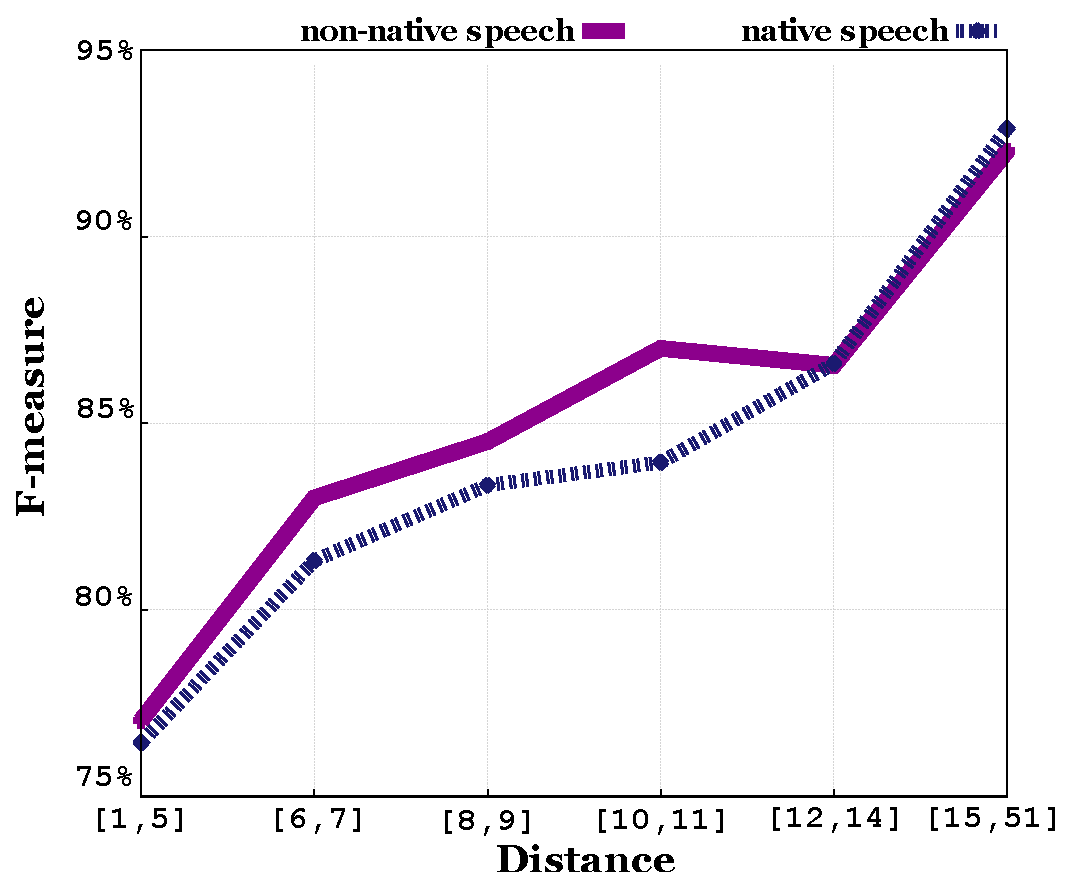
\includegraphics[scale=0.25]{Image/allStats_curve} 
\par\end{centering}

\caption{Overall performance}
\label{Figure:perform}
\end{figure}



\section{Conclusions}

This paper studied the rejection of incorrect entries, with a focus
on non-native speech, in the context of foreign language learning.

Assessments carried out on two English corpora (one native and one
non-native) have shown that it is important to train the decision
functions on the same type of data (native training for tests on native
speech, non-native training for tests on non-native speech). The use
of alternative non-native pronunciations in the lexicon is necessary
only for the task of non-native transcript verification. It is also
useful to combine all comparison criteria (i.e. from both the phoneme
loop and the word loop segmentations) through a logistic regression
function which assigns weights according to the importance of each
criterion.

The optimal settings lead to reasonable false acceptance and false
rejection error-rates (1.80\% and 1.29\%, corresponding to a F-measure
of about 98\%, for non-native data, 8.84\% and 2.49\%, corresponding
to a F-measure of about 94\%, for native data) when the pronounced
sentences are entirely different from the expected sentences. For
partially different sentences, starting from a distance of 6 phoneme
changes we can obtain a performance greater than 80\%.  
\bibliographystyle{IEEEbib}
\bibliography{biblioSTL}

\end{document}
